\begin{mdframed}[style=warning]
	\textbf{Conceptos}
		\begin{enumerate}
			\item La rapidez vertical de un segmento de una cuerda tensa horizontal, a través de la que viaja una onda, ¿depende de la rapidez de al onda?
			\item Dos ondas viajan en la misma cuerda. ¿Es posible para ambas tener $a)$ diferentes frecuencias, $b)$ diferentes longitudes de onda, $c)$ diferentes rapideces, $d)$ diferentes amplitudes, $e)$ la misma frecuencia, pero diferentes longitudes de onda? Explique su razonamiento.
		\end{enumerate}
\end{mdframed}



















\begin{mdframed}[style=warning]
	\begin{ejercicio}
		Una onda sonora senoidal pura se describe matemáticamente por la siguiente función
			$$ S(x,t) = 3\times 10^{-6} \sin{\qty(2\pi x + 680\pi t)}. $$
		Donde $S(x,t)$ es el desplazamiento de las partículas a partir de su posición de equilibrio. La expresión esta dada en el SI. Esta onda se propaga en el aire cuya densidad es $\rho = 1..21kg/m^3$. Calcule
		\begin{multicols}{2}
			\begin{enumerate}[a)]
				\item La amplitud de esta onda.
				\item La velocidad de onda.
				\item La dirección de la propagación.
				\item El número de onda.
				\item La longitud de onda.
				\item La frecuencia.
				\item La amplitud de cambio de presión.
				\item La intensidad y su nivel sonoro.
			\end{enumerate}
		\end{multicols}
	\end{ejercicio}
\end{mdframed}


























\begin{mdframed}[style=warning]
	\begin{ejercicio}
		En la figura se tiene un alambre de alumninio de longitud $L_1 = 60cm$, con área de sección transversal $1\times 10^{-2} cm^2$, y con densidad $2.6g/cm^3$, está unido a un alambre de acero, de densidad $7.8g/cm^3$ y la misma área de sección transversal. El alambre combinado, cargado con un bloque de masa $m = 10kg$, se configura para que la distancia $L_2$ medida desde el punto de unión a la polea de soporte sea de $86.6cm$. Se establecen ondas transversales en el alamabre por una funete externa de frecuencia variable; un nodo se localica en la polea. Encuentre:
		\begin{enumerate}[a)]
			\item La frecuencia más baja que genera una onda estacionaria teniendo el punto de unión como uno de los nodos.
			\item ¿Cuántos nodos se observan a esa frecuencia?
		\end{enumerate}
		
		\begin{figure}[H]
			\centering
			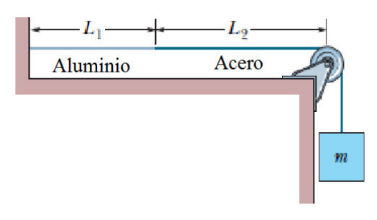
\includegraphics[scale=0.4]{./img/alambres.png}
			\caption{\centering Configuración de los alambres.}
			\label{ej4}
		\end{figure}
	\end{ejercicio}
\end{mdframed}









































%%%